%\chapter{Úvod}\label{chap:intro}

\chapter{Východiská}\label{chap:intro}

\section{UNITY}

Unity vychádza z knihy Parallel Program Design - A Foundation, v ktorej bol Unity popísaný a navrhnutý autormi K. Mali Chandy a Jayadev Misra z Univerzity of Texax.



\section{Vlastnosti UNITY}

\begin{itemize}
\item Nedeterminizmus
\item Absencia toku riadenia (control-flow)
\item Synchrónnosť a asynchrónnosť
\item Stavy a priradenia
\end{itemize}


\subsection{Nedeterminizmus}
...

\subsection{Absencia toku riadenia (control-flow)}
...

\subsection{Synchrónnosť a asynchrónnosť}
...

\subsection{Stavy a priradenia}
...

\section{Telo programu}

Unity obsahuje štyri základné sekcie: decleráciu premmenných, množinu skratiek, počiatočné hodnoty premenných a množinu priraďovacích príkazov. V tele programu sa tieto sekcie vyskytujú pod názvamy declare, always, initially, assign. Telo programu obsahuje aj program-name, názov programu, ktorý môžeme vynechať, v tom prípade z tela programu vynechávame aj sekciu program-name. Unity program má nasledujúcu formu:

\begin{figure}[h]
\centerline{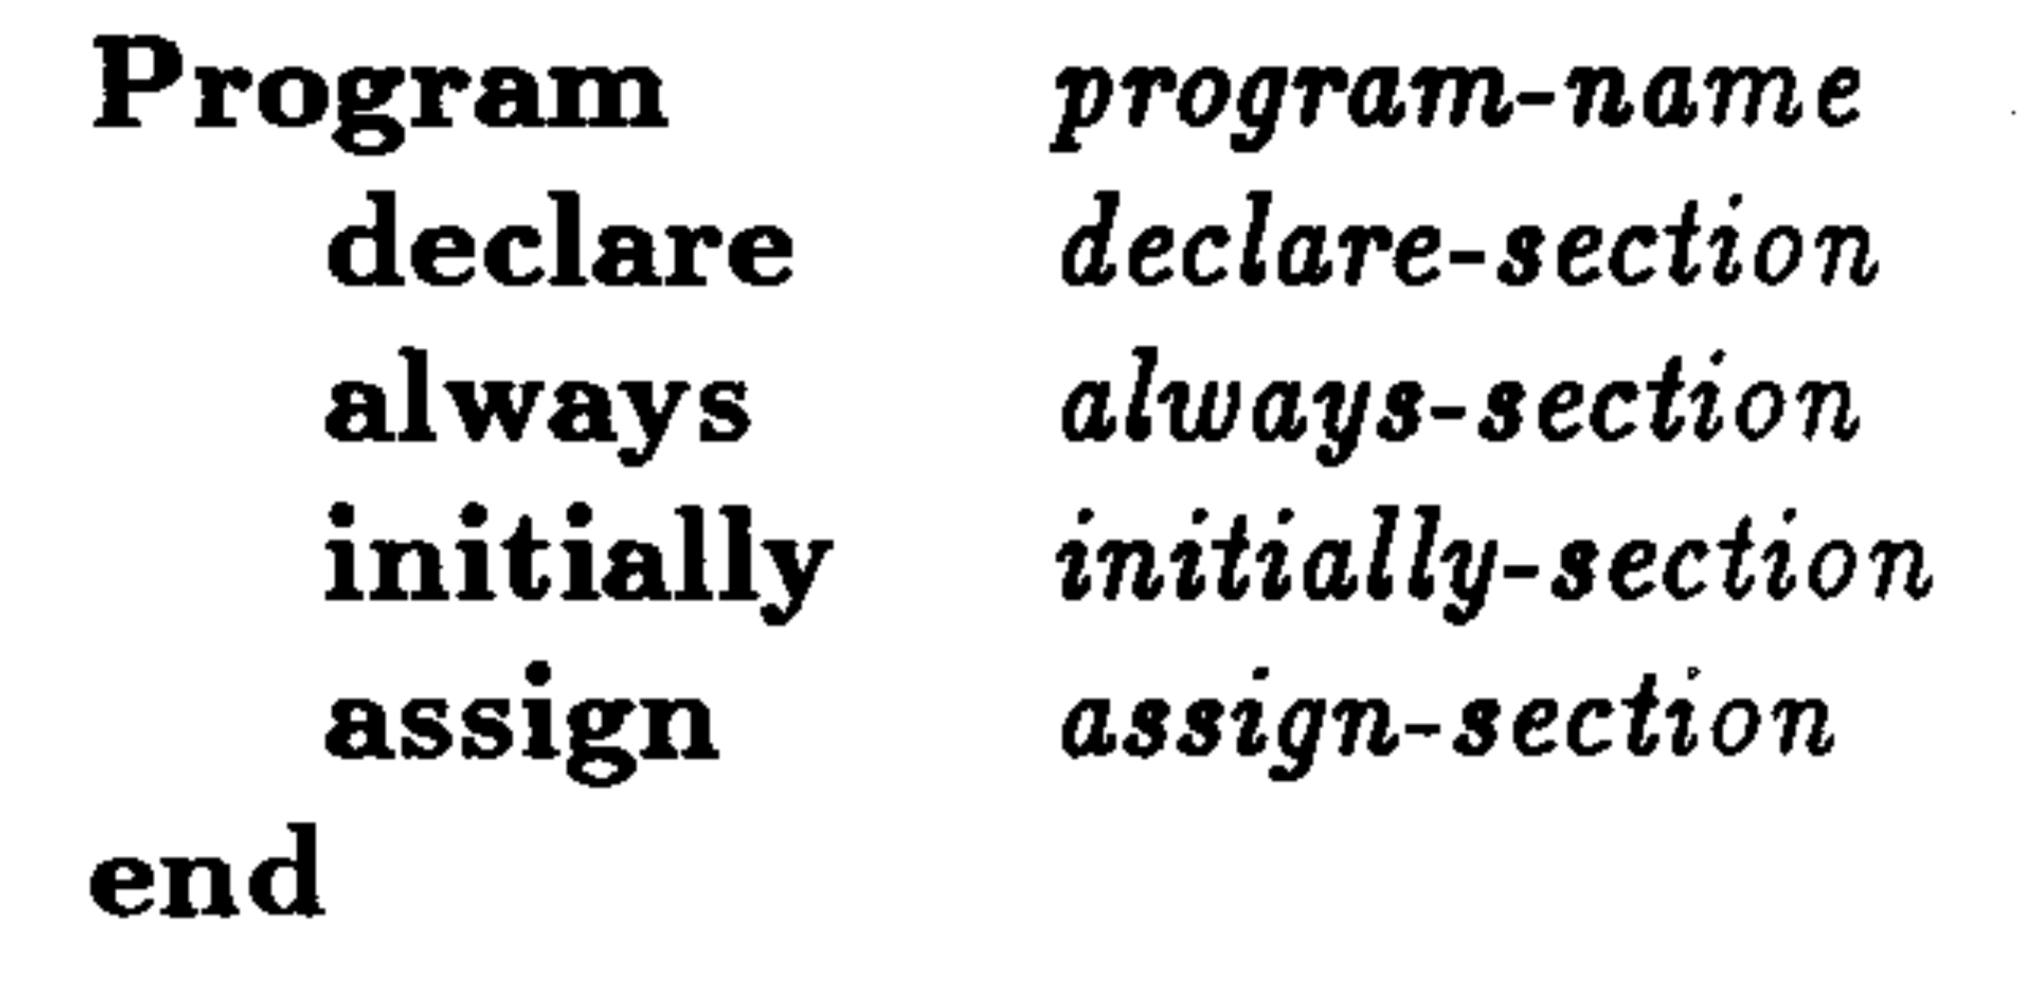
\includegraphics[width=0.6\textwidth]{images/screen1}}
\caption[Ukážka tela programu]{Ukážka tela programu}
\label{obr:programbody}
\end{figure}

\subsection{Declare-section}

Táto sekcia obsahuje dekleráciu premenných použité v programe a ich súvisiace typy. V nasledujúcej ukážke môžete vidieť dekleráciu premenných x a y typu integer. Syntax je podobná ako v programovacom jazyku PASCAL. 

\vspace{5mm}

Medzi základné typy patria:
\begin{itemize}
\item Integer
\item Boolean
\end{itemize}

\vspace{5mm}

Príklad deklerácie:
\begin{lstlisting}
declare 
	x, y : integer
\end{lstlisting}

\vspace{5mm}

Taktiež sa využívajú n-rozmerné polia v nasledujúcom tvare:
\begin{lstlisting} d
declare 
	p: Array[a1, a2, ..., an] of integer
\end{lstlisting}

\subsection{Always-section}

Sekcia always definuje skratky, ktoré slúžia na stručné spísanie programu. Konkrétnejšie to sú premenné, ktoré definujú funkcie alebo podmienky. Takéto premenné sú známe ako transparentné premenné. Transparentné premenné poskytujú vhodný spôsob skrátenia výrazov, ktoré sa často vyskytujú v programe. Táto sekcia nie je nevyhnutná v tele programu Unity. 

Transparentné premenné môžeme definovať následovne pomocou ||:
\begin{lstlisting}
always
		decx = x > y
	||
		decy = y > z
\end{lstlisting}
Tieto premenné je možné zapísať aj jednoriadkovo bez použitia spojovníka:

\begin{lstlisting}
always
	decx, decy = z > y, y > z
\end{lstlisting}

\subsection{Initially-section}

Initially sekcia je súbor rovníc, ktoré definujú počiatočné hodnoty pre niektoré programové premenné. Premenné, ktoré nie sú inicializované majú ľubovoľné počiatočné hodnoty. Premenné x a y môže byť definované:

\begin{lstlisting}
initially
		x = X
	||
		y = Y
\end{lstlisting}

alebo takto:

\begin{lstlisting}
initially
	x, y = X, Y
\end{lstlisting}
\subsection{Assign-section}


\subsection{Ukážka programu}
Nasledujúci Unity program predsavuje Euclidovský algoritmus pre nájdenie najväčšieho spoločného deliteľa čísel X, Y:
\begin{figure}[h]
\centerline{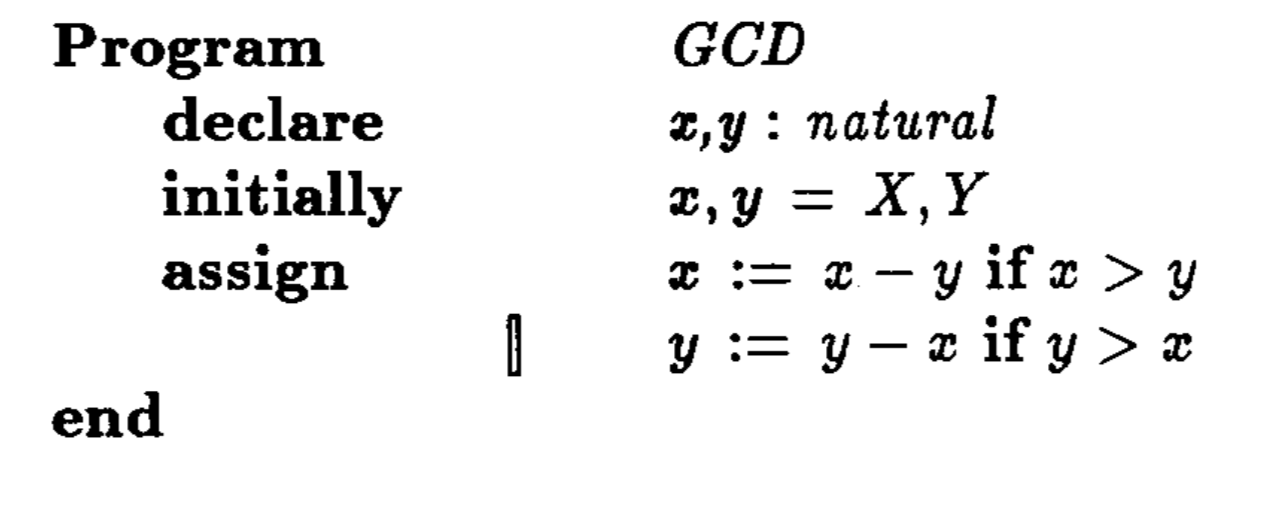
\includegraphics[width=0.7\textwidth]{images/screen2}}
\caption[GCD algoritmus]{GCD algoritmus}
\label{obr:gcd}
\end{figure}

\section{Syntaktický strom}

\section{Syntaktická analýza}

\section{Model checking}

\section{LTSmin}

\subsection{Back-ends}

\subsection{Front-ends}